
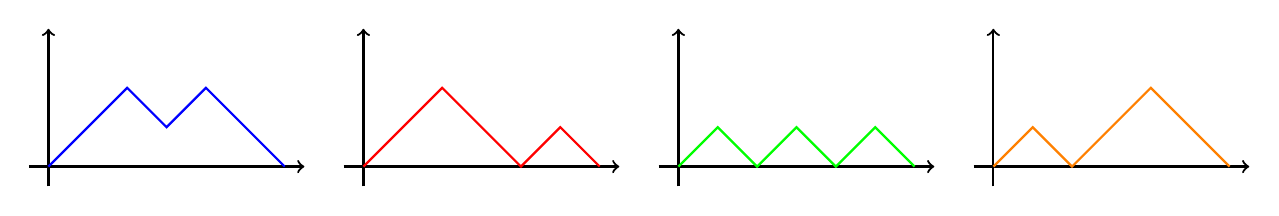
\begin{tikzpicture}[scale=0.5]

    % Dessin des chemins de Dyck pour n = 3, alignés horizontalement

    % Chemin 1
    \begin{scope}[shift={(0,0)}]
        \draw[->,thick] (-0.5,0) -- (6.5,0); % Axe horizontal
        \draw[->,thick] (0,-0.5) -- (0,3.5); % Axe vertical
        \draw[thick, blue] (0,0) -- (1,1) -- (2,2) -- (3,1) -- (4,2) -- (5,1) -- (6,0);
    \end{scope}

    % Chemin 2
    \begin{scope}[shift={(8,0)}]
        \draw[->,thick] (-0.5,0) -- (6.5,0); % Axe horizontal
        \draw[->,thick] (0,-0.5) -- (0,3.5); % Axe vertical
        \draw[thick, red] (0,0) -- (1,1) -- (2,2) -- (3,1) -- (4,0) -- (5,1) -- (6,0);
    \end{scope}

    % Chemin 3
    \begin{scope}[shift={(16,0)}]
        \draw[->,thick] (-0.5,0) -- (6.5,0); % Axe horizontal
        \draw[->,thick] (0,-0.5) -- (0,3.5); % Axe vertical
        \draw[thick, green] (0,0) -- (1,1) -- (2,0) -- (3,1) -- (4,0) -- (5,1) -- (6,0);
    \end{scope}

    % Chemin 4
    \begin{scope}[shift={(24,0)}]
        \draw[->,thick] (-0.5,0) -- (6.5,0); % Axe horizontal
        \draw[->,thick] (0,-0.5) -- (0,3.5); % Axe vertical
        \draw[thick, orange] (0,0) -- (1,1) -- (2,0) -- (3,1) -- (4,2) -- (5,1) -- (6,0);
    \end{scope}


\end{tikzpicture}
